\chapter{Human Pose Estimation (HPE)}
\vspace{-1cm}
\begin{figure}[h]
    \centering
    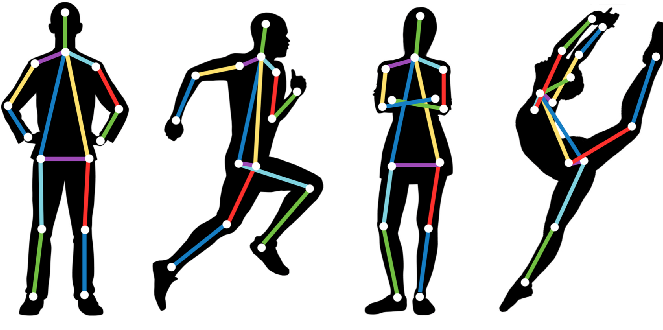
\includegraphics[scale=0.7]{img/hpe.png}
\end{figure}

\vspace{-0.5cm}
\section{Introduction, motivations and challenges}
\textbf{Human Pose Estimation (HPE)} deals with the estimation of the position of one or more human body within an image. HPE focuses on static body poses in individual frames, while HAR we have explained in the previous chapter looks at dynamic movement patterns across the video. How we will see at the end, human pose estimation can be used as input feature for HAR.
\vspace{-0.6cm}
\subsection{Applications of HPE}
The \textbf{applications} that HPE can find are: \textit{HCI} (Human-Computer Interaction), \textit{Virtual reality}, for realizing special effects in \textit{movies and animation}, sport motion analysis and also for video survelillance combined with HAR tasks.
\vspace{-0.5cm}
\subsection{Challenges related to Human Pose Estimation}
Like HAR, also HPE is a \textbf{very challenging computer vision task} for several reasons: (i) the human body is extremely flexible (high DOF), it suffer from self-occlusions (that is parts which are superimposed)...\\
\noindent
The \textbf{basic steps} are mainly: 
\begin{enumerate}
    \itemsep-0.3em
    \item Localizing human body (SPPE) or human bodies (MPPE) \textbf{joints/keypoints}; 
    \item Grouping them together into \textbf{valid configurations}.
\end{enumerate}

How you can imagine the problem of estimating the pose of multiple people within a scene is even more complicate. We will proceed step-by-step in the explanation analyzing the most popular models from simpler ones to achieve more complicate architectures.

\section{Single-Person Pose Estimation (SPPE)}

\subsection{DeepPose}
\textbf{DeepPose} is historically the first model which uses ConvNets for HPE. This model was introduced in \citedate{Toshev_2014} in the paper \citetitle{Toshev_2014}, \cite{Toshev_2014}. The problem of detecting the body joints is cast as a \textbf{DNN-based regression problem}, then the outputs are 2D body joint positions. A multi-stage architecture is implemented for prediction refinement and an \textit{holistic approach} is used in the sense that all joints are estimated even if not visible.

\subsubsection{DeepPose architecture}
\begin{figure}[h]
    \centering
    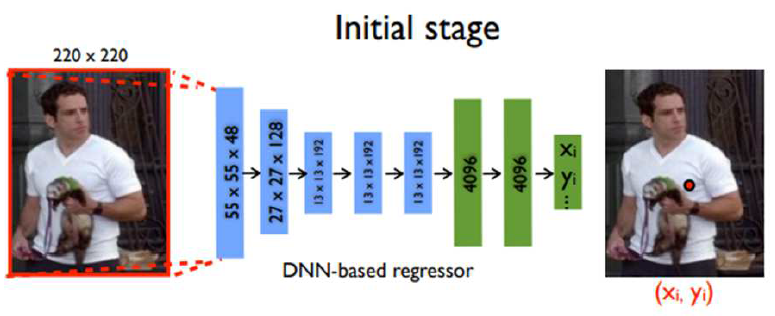
\includegraphics[scale=0.7]{img/DeepPose.png}
    \caption{DeepPose initial stage}
\end{figure}
The first step is an \textit{image preprocessing}, an object detector is used in order to find the person within the image; the original image, is then cropped taking as reference the bounding box information. As DNN backbone is used AlexNet, with an extra laye for predicting the (x,y) position of $k$ body joints. Since this is a regression task, a least-squares based loss can be used for training it. \\
After this initial stage, the estimated pose is passed through a cascade of three regressors in order to refine it by cropping the original image around the predicted point and passing it to the next-step regressor.
\vspace{-0.5cm}
\begin{figure}[h]
    \centering 
    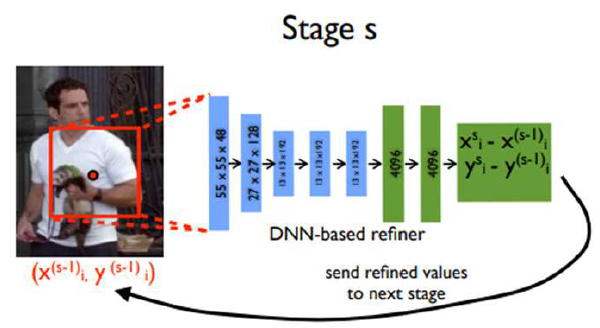
\includegraphics[scale=0.8]{img/DeepPose2.png}
    \caption{DeepPose: estimated pose refinement}
\end{figure}
DeepPose is the first CNN-based approach for estimating the pose of a single human body within a scene. The main limitation is that regressing joint positions is an extremely difficult task. More specifically, only regression is not sufficient to effectively solve the SPPE task. 


\subsection{ConvNet Pose: toward the use of heatmaps}
At this stage, after having introduced the first model, is shift the problem to the estimation of \textbf{heatmaps for joints} and then find coordinates as a second step according to the regions of major activation.
\begin{definition}[\textbf{Heatmap}]
    Given a joint, its heatmap is an \textit{image} where each pixel contains the probability that the joint is located there.
\end{definition}
\begin{figure}[h]
    \centering
    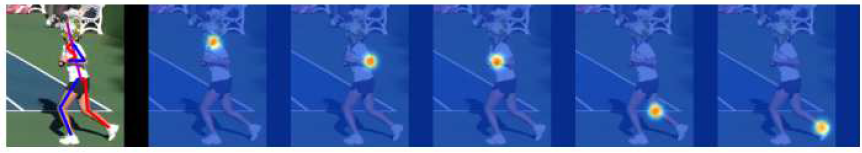
\includegraphics[scale=0.8]{img/HeatMap.png}
    \caption{Joints on a runner with related heatmaps}
\end{figure}

One of the first approaches for the computations of HeatMaps is presented in \citetitle{ConvNetPose} (\citeauthor{ConvNetPose}, \cite{ConvNetPose}) where a \textit{multiscale filtering approach} is used. The idea of refining predictions is kept from DeepPose and reused by following works on HPE.\\
\subsubsection{ConvNet Pose approach}
The model proposed in \cite{ConvNetPose}, follows a sliding-window approach, in particular it analyzes \textbf{three pyramidal versions} of the input and produces a \textit{coarse estimation} for both heatmaps and joint locations $(x,y)$. Such joint estimates are used to crop the features of the first conv layer which are fed 

\subsection{Convolutional pose machines (CPM)}

\section{Multiple-Person Pose Estimation(MPPE)}

\subsection{OpenPose}

\subsection{DeepCut}

\subsection{AlphaPose (RMPE): a top-down approach}


